\label{user-manual}

\section*{A graphical user interface for DARWIN}

\subsection*{Starting the GUI application}

A runnable jar with all the required dependencies is provided. See the disc
attached to the thesis. The distribution is also available on-line at
\url{http://github.com/downloads/puszczyk/DarwinDS/distribution.zip}. The Java
Runtime Environment (JRE) 1.5 or later is required. To run the application,
double click on a~file \texttt{darwin-full.jar} in a~graphical user interface
or type following command in a terminal:\\
\texttt{\$ java -jar darwin-full.jar} \\
The figure~\ref{manual_01_main} shows the main window of DARWIN.

\begin{figure}[htb]
  \centering
  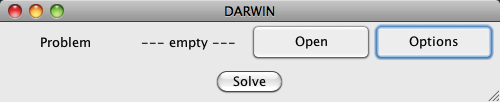
\includegraphics[scale=0.7]{img/manual/01_main_screen}
  \caption{The main screen of DARWIN}
  \label{manual_01_main}
\end{figure}

A set of problems (the ones with uncertain values) is included with the
distribution.

\subsection*{Solving exemplary problems}

DARWIN offers an intuitive and easy to use interface for solving MMO
problems. The main window is presented in figure~\ref{manual_01_main}. To
solve a~problem one need to execute following steps:

\begin{enumerate}
\item Click the ``Open'' button in the main window.
\item Choose a problem file using a~provided file selector
  (fig.~\ref{manual_02_problem_selector}). The problem has to be described in
  the DARWIN .mod (model) file format.
\item The main window now shows a name of the problem
  (fig.~\ref{manual_03_selected}). Click ``Solve''.
\item A window presenting generated solutions appears
  (fig.~\ref{manual_04_mark_as_good}). Mark preferred solutions as ``good''
  using checkboxes in the ``is good'' column.
\item A window with solution details can be invoked by selecting a~solution
  and clicking the ``Solution details'' button (fig.~\ref{manual_05_dec_var}).
\item After selecting the solutions an evolutionary optimization begins
  (fig.~\ref{manual_06_evo_loop}). New solutions are generated and one can
  mark ``good'' solutions from a new set again.
\item If generated solutions are satisfactory, then one can stop the
  algorithm by clicking ``Mark as good'' when no solutions are selected
  (fig.~\ref{manual_07_finish}).
\end{enumerate}

\begin{figure}[htb]
  \centering
  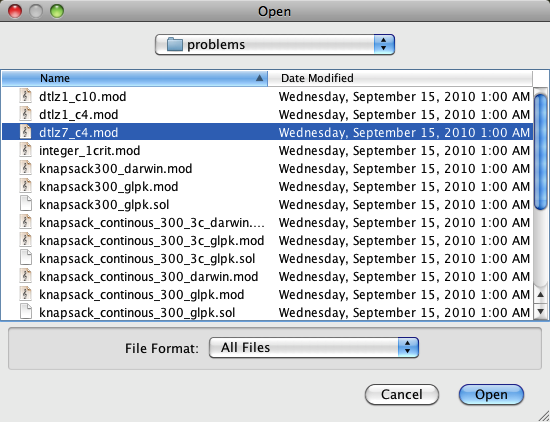
\includegraphics[scale=0.7]{img/manual/02_problem_selector}
  \caption{Selecting a problem to solve}
  \label{manual_02_problem_selector}
\end{figure}

\begin{figure}[htb]
  \centering
  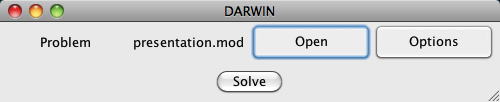
\includegraphics[scale=0.7]{img/manual/03_problem_selected}
  \caption{Starting the algorithm}
  \label{manual_03_selected}
\end{figure}

\begin{figure}
  \centering
  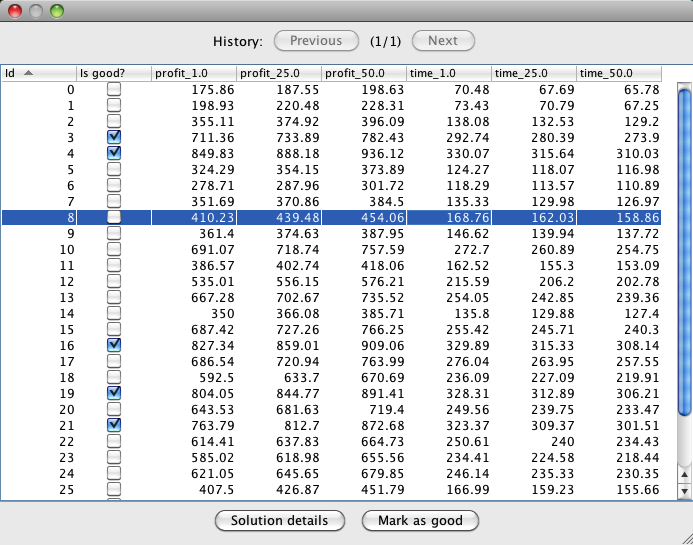
\includegraphics[scale=0.7]{img/manual/04_marking_solutions}
  \caption{Marking the ``good'' subset of generated solutions}
  \label{manual_04_mark_as_good}
\end{figure}

\begin{figure}
  \centering
  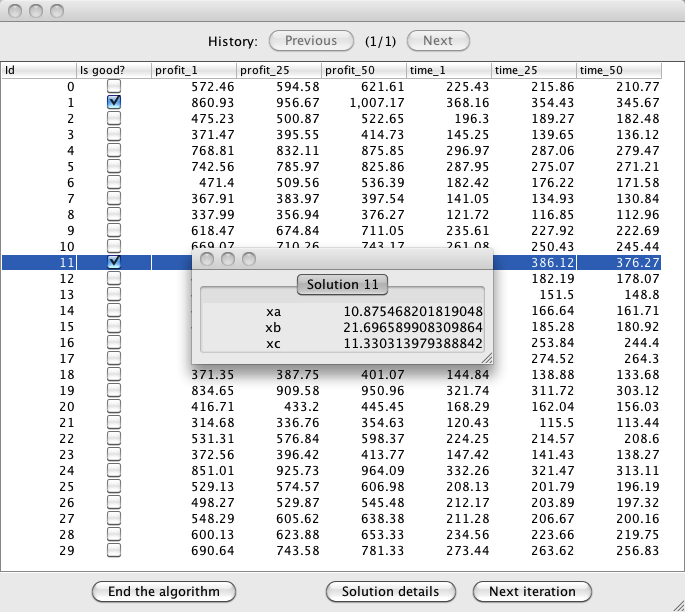
\includegraphics[scale=0.7]{img/manual/05_solution_details}
  \caption{Decision variables for a given solution}
  \label{manual_05_dec_var}
\end{figure}

\begin{figure}
  \centering
  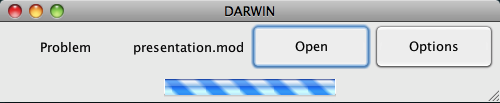
\includegraphics[scale=0.7]{img/manual/06_evolutionary_loop}
  \caption{An evolutionary optimization is performed}
  \label{manual_06_evo_loop}
\end{figure}

\begin{figure}
  \centering
  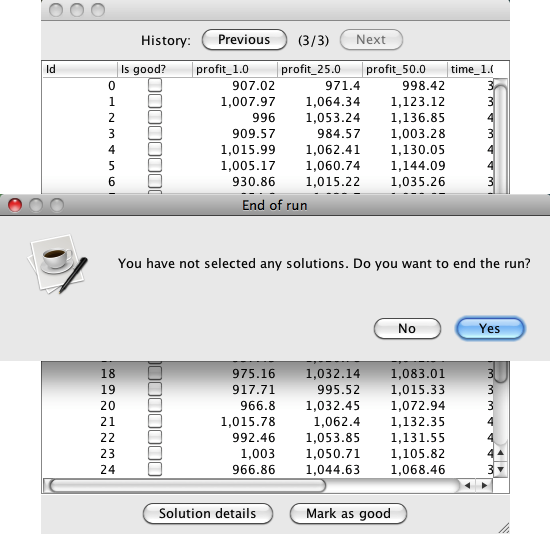
\includegraphics[scale=0.7]{img/manual/07_end_of_run}
  \caption{Finish the problem analysis}
  \label{manual_07_finish}
\end{figure}

\clearpage{}
\subsection*{Advanced options}

The DARWIN GUI offers additional options to customize the process. One can
modify the algorithm parameters in a~configuration dialog
(fig.~\ref{manual_08_options}). To open it, click the ``Options'' button in
the main window. The options are described below.

\begin{table}[htb]
  \centering
  \begin{tabular}{l p{3.5cm} p{6.5cm} l l}
    \hline
    Tab & Option name & Description & Default value \\
    \hline
    \hline
    \multirow{5}{*}{Main}
    & The number of solutions & The number of solutions in a population. & 30 \\
    & The number of scenarios & The number of scenarios on which the solutions will be evaluated.  & 30 \\
    & The number of generations & The number of generations in the interior loop. & 30 \\
    & Percentiles & Which percentiles are meaningful to the decision maker. & 1.0, 25.0, 50.0  \\
    & Use an average in quantiles & Whether an average in quantiles should be used instead of
    the maximum value. & false  \\
    \hline
    \multirow{3}{*}{The Algorithm}
    & Use All Rules instead of DomLem & Should the All Rules algorithm be used
    instead of the default one & false \\
    & The DomLEM confidence level & A level of confidence which the rules generated by the
    DomLem algorithm should at least have. & 0.6 \\
    & Compare using the supposed utility function & If the evolutionary algorithm should use the
    supposed utility instead of a rule-based score. & false \\
    \hline
    \multirow{4}{*}{Fine Tuning} 
    & Delta & The decay of the rule weight (see \ref{idea-algo}). & 0.1  \\
    & Gamma & The coefficient of an elitism. The higher the gamma, the
    higher the probability of choosing a solution with a~higher rank as
    a~parent. & 2.0  \\ 
    & Eta & The initial mutation probability.  & 0.5    \\
    & Omega & The decay rate of the mutation probability. & 0.1  \\
    \hline
    \multirow{5}{*}{Reports} 
    & The reports directory & A directory where reports should be saved. &
    ./reports  \\
    & Save the evolutionary report & If the evolutionary report should be
    saved ia a~file. & false \\
    & Save the decision maker's report & If the DM's report should be
    saved in a~file. & false \\
    & The rules directory & A directory where rules should be saved. &
    ./rules  \\
    & Save rules & If the decision rules generated during a run should be
    saved on a~disk. & false \\
    \hline
    \multirow{1}{*}{GUI Parameters}
    & Digits after a dot & A number of digits that should be displayed after a
    dot. & 2 \\    
    \hline
  \end{tabular}
\end{table}


The window presenting a~list of generated solutions offers additional
features. The list of solutions can be sorted on a given criterion by clicking
the column header (fig.~\ref{manual_09_sorton}). Another useful option is a
history of solutions. The user can review solutions generated in earlier
iterations, return to them and change his or her selections. This is possible
using the history toolbar (see\ref{manual_10_history}).

\begin{figure}
  \centering
  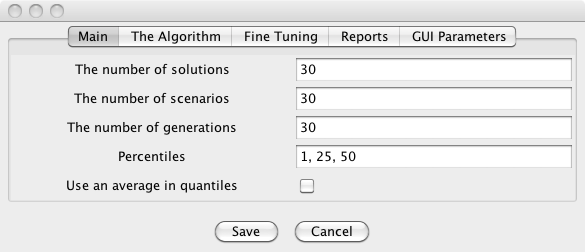
\includegraphics[scale=0.7]{img/manual/08_options}
  \caption{DARWIN configuration options}
  \label{manual_08_options}
\end{figure}

\begin{figure}
  \centering
  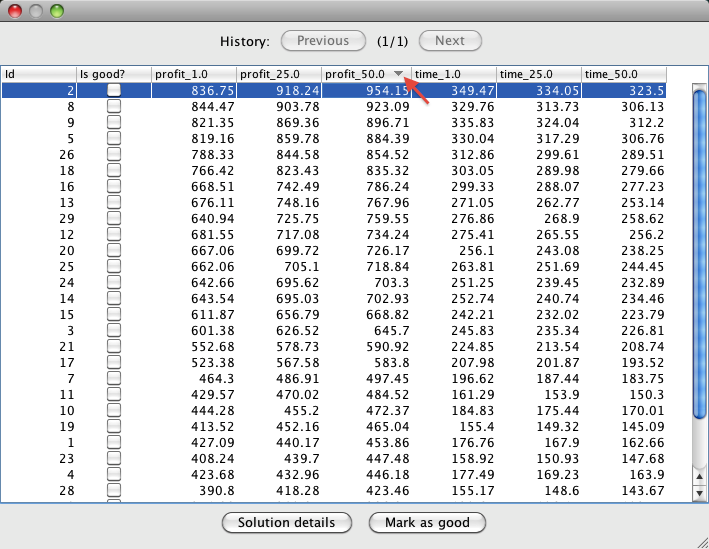
\includegraphics[scale=0.7]{img/manual/09_sorton}
  \caption{Sorting solutions on a given criterion}
  \label{manual_09_sorton}
\end{figure}

\begin{figure}
  \centering
  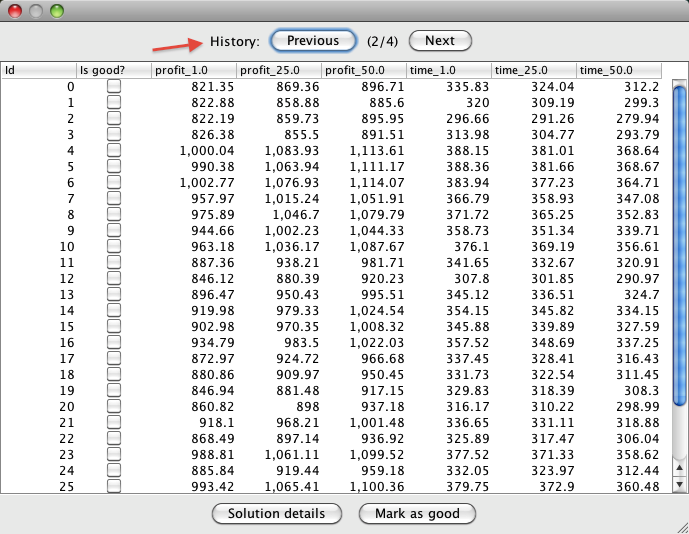
\includegraphics[scale=0.7]{img/manual/10_history}
  \caption{Reviewing the history of generated solutions}
  \label{manual_10_history}
\end{figure}

\clearpage{}
\section*{The DARWIN .mod file format}

MMO problems for DARWIN are specified in external files. These files are
called the DARWIN model files and usually have the \texttt{.mod}
extension. The application contains a~parser for the model files. The parser
grammar in the Extended Backus-Naur Form (EBNF, see~\cite{Wir77}) is described
below.

\lstinputlisting{res/parser.txt}

Comments handled by a~preprocessor are possible --- (1) line comments,
starting with \texttt{\#}, e.g. \texttt{ \#a-line-comment} and (2) block
comments, enclosed in \texttt{/* */}. Whitespaces are ignored.

A problem file consists of lines, each line contains a~statement ended by
a~semicolon (\texttt{;}). A statement can define the supposed utility
function, a~variable, a~goal or a~constraint. The variables are defining the
problem domain. They can be continuous (with double floating point precision),
binary (indicated by a \texttt{(B)} flag) or integer (\texttt{(I)} flag).
Upper and lower limits of the variable value have to be provided. Each
variable has a name and can be referred by the name in succeeding
statements. Goals are the optimization criteria to be minimized or
maximized. They are named expressions and therefore can be referred later by
the name. Constraints are named inequalities. The inequality is not strict and
both its sides can be expressions. Finally, the supposed utility function is
an expression prefixed with \texttt{!dec:}. The function is useful only if one
wants to mock the decision maker.

An example file with the mix-problem definition is included below.

\lstinputlisting{res/presentation.mod}

The expressions are utilizing intervals (e.g. \texttt{[pa:20, 24]}) and the
supposed utility function is using meaningful percentiles
(e.g. profit$^{25\%}$: \texttt{<profit, 0.25>}).



\section*{Compiling DARWIN from the source code}

It is possible to build a DARWIN binary from the source code. It can be done
using command line on Windows, Linux and MacOSX.  Instructions are given
below.

\begin{enumerate}

\item \textbf{Get the source code}. Sources are included in a~disk attached to
  the thesis. Alternatively, most recent version is stored in the git
  repository (see~\cite{Loe09})  and can be cloned by typing a~command:\\
  \texttt{\$ git clone git://github.com/puszczyk/DarwinDS.git}
\item \textbf{Prepare a build tool}. DARWIN uses sbt (see~\cite{sbt10})---
  a~build tool for Scala. Detailed setup instructions are given in the
  project's webpage. The easiest way is to install Scala (system-dependent,
  consult \url{http://scala-lang.org} for details) and then prepare a script
  for running sbt. Download sbt-launch.jar from the sbt website:
  \url{http://simple-build-tool.googlecode.com/files/sbt-launch-0.7.4.jar}
  \\
  Somewhere in the \text{PATH} put a script with the following content: \\
  \texttt{java -Xmx512M -jar `dirname \$0`/sbt-launch.jar "\$@"} \\
  or (in case of Windows operating system): \\
  \texttt{set SCRIPT\_DIR=\%~dp0} \\
  \texttt{java -Xmx512M -jar "\%SCRIPT\_DIR\%sbt-launch.jar" \%*} \\
  Make the file executable. It is assumed further, that the script is named
  \texttt{sbt}.
\item \textbf{Build the DARWIN binaries}. Source code is located in the
  \texttt{Darwin} directory. First get required dependencies: \\
  \texttt{\$ cd DarwinDS/Darwin} \\
  \texttt{\$ sbt} \\
  \texttt{> download-jars} \\
  Then run a set of unit-test to check if everything went fine up to this
  point:\\
  \texttt{> test} \\
  This should end with a~message: \\
  \texttt{[info] All tests PASSED.} \\
  \texttt{[success] Successful.} \\
  Now DARWIN can be compiled: \\
  \texttt{> compile} \\
  And run: \\
  \texttt{> run} \\
  To create a \texttt{.jar} package type: \\
  \texttt{> package} \\
  This will generate DARWIN binaries in a subdirectory named \texttt{target}.
\end{enumerate}


\section*{The experiment framework} 

Instead of a graphical user interface, DARWIN can be run in a~console-based
batch mode. This is useful for running a~set of experiments. The batch run can
be invoked by the experiment framework located in the \texttt{Experiment}
directory. The directory contains a few useful scripts written in Bash and
Python. As such it requirers MacOSX or a Linux distribution or a Windows
operating system with Cygwin installed (see~\cite{Laz00}). The utility scripts
are described below:

\begin{itemize}
\item \texttt{runTestPlan.py} --- a script for running a~set of tests. As an
  input it requires a location of the DARWIN directory, a~problem file,
  a~darwin configuration file and a~test plan specification. The problem file
  is a file in the DARWIN .mod file format. The configuration is an .ini file
  structured as follows:
  \begin{lstlisting}
    [section]
    option1 = value1
    option2 = value2
    (...)
    optionN = valueN
  \end{lstlisting}

  
  Required sections and options are described in the table~\ref{t:params}. The
  test plan specification is a text file with the~following structure:
  \begin{lstlisting}
    >test_name_1/number-of-runs
    [section-to-override]
    option-to-override1 = value1
    (...)
    >test_name_N/number-of-runs
    (...)
  \end{lstlisting}

  Each test is run \texttt{number-of-runs} times. For each test one can
  specify a~list of options to be overridden. It is useful for testing an
  influence of a parameter. An example test plan is presented below.
  \begin{lstlisting}
    >delta005/15
    [main]
    delta = 0.05

    >delta015/15
    [main]
    delta = 0.15

    >delta020/15
    [main]
    delta = 0.20

    >delta040/15
    [main]
    delta = 0.40
  \end{lstlisting}

  This plan will run DARWIN fifteen times for each \texttt{delta} value. Run
  reports are saved in a~directory named after the current date and time. Test
  names are the names of subdirectories.

\item \texttt{genCharts.sh} --- a script for charting run reports. It requires
  installing the \texttt{R} environment (see~\cite{kee10}) with
  \texttt{ggplot2} and \texttt{reshape} libraries. The charts to be generated
  are included in the
  \texttt{Chart} directory of the DARWIN distribution. The usage is: \\
  \texttt{\$ genCharts.sh --brief/--full criteria-no best-val charts-dir
    testplan-out-dir} \\
  \texttt{--brief/--full} decides whether all charts or only the overview
  chart should be generated. \texttt{criteria-no} is the~number of criteria in
  the problem. \texttt{best-val} --- an optimal value of the problem, if can
  not be given should be set to $0$. \texttt{charts-dir} is the directory with
  the \texttt{R} charts to be generated. Finally, \texttt{testplan-out-dir} is
  an output directory of the \texttt{runTestPlan.py} script. Available types
  of charts are presented in figure~\ref{chart_examples}.

  The script will generate distinct charts for each test run. If one wants a
  comparison between the tests, then \texttt{./genSummaryChart.sh} should be
  used instead.

\item \texttt{genSummaryChart.sh} --- a script for charting a comparison
  between different test runs. The usage is similar to \texttt{genCharts.sh},
  however the number of criteria can be omitted, because is irrelevant to the
  task. The usage is: \\
  \texttt{\$ ./genSummaryChart.sh best-val charts-dir testplan-out-dir
    problem-name}\\
  Available types of charts are presented in figure~\ref{chart_examples2}.



\end{itemize}


%%% Local Variables: 
%%% mode: latex
%%% TeX-master: "main"
%%% End: 
